\chapter{Solution Transfer}\label{chap:solution-transfer}

\section{Introduction}

In this chapter, an algorithm for conservative solution transfer between curved
meshes will be described. This has practical applications to many methods in
computational physics. Solution transfer is needed when a solution
(approximated by a discrete field) is known on a \emph{donor} mesh and must
be transferred to a \emph{target} mesh. In many applications, the field
must be conserved for physical reasons, e.g. mass or energy cannot leave or
enter the system, hence the focus on \emph{conservative} solution transfer.
A few scenarios where solution transfer is necessary will be considered below
to motivate the ``black box'' solution transfer algorithm.

Since solution transfer is so commonly needed in physical applications, this
problem of conservative interpolation has been considered already for
straight sided meshes. The \emph{common refinement} approach in
\cite{Jiao2004} is used to compare several methods for solution transfer across
two meshes. However, the problem of constructing a common refinement is
not discussed there. The problem of constructing such a refinement is
considered in \cite{Farrell2009, Farrell2011} (called a supermesh by
the authors).
However, the solution transfer becomes considerably more challenging for curved
meshes. For a sense of the difference between the straight sided and curved
cases, consider the problem of intersecting an element from the donor mesh
with an element from the target mesh. If the elements are triangles, the
intersection is either a convex polygon or has measure zero. If the elements
are curved, the intersection can be non-convex and can even split into
multiple disjoint regions.

\subsection{Lagrangian Methods}

\begin{figure}
  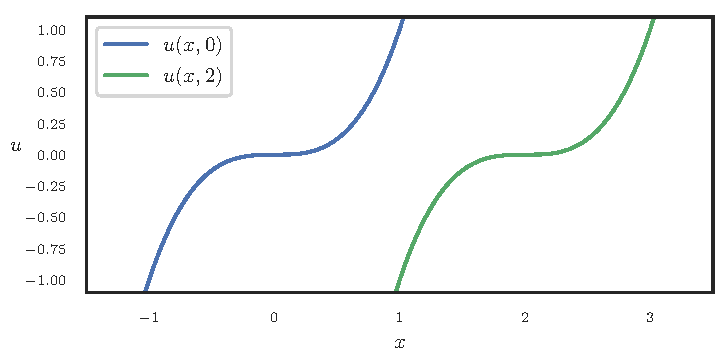
\includegraphics{../images/solution-transfer/simple_transport.pdf}
  \centering
  \captionsetup{width=.75\linewidth}
  \caption{The solution to \(u_t + u_x = 0, \; u(x, 0) = x^3\) plotted in
    the \(xu\)-plane. Demonstrates simple transport of
    the solution.}
  \label{fig:simple-transport}
\end{figure}

The method of characteristics helps transform partial differential equations
into ordinary differential equations by dividing the physical domain into
a family of curves. For example, the simple transport equation
\begin{equation}\label{eq:simple-transport}
u_t + c u_x = 0
\end{equation}
can be transformed when restricting to the family of lines
\(x(t) = x_0 + c t\). On these lines \(u(x(t), t)\) is constant, by
construction, and so the solution is ``transported'' from \(u(x_0, 0)\)
along each characteristic line (Figure~\ref{fig:simple-transport}).

Motivated by this, \emph{Lagrangian methods} treat each point in the
physical domain as a ``particle'' which moves along a characteristic curve
over time and then monitor values associated with the particle (heat / energy,
velocity, pressure, density, concentration, etc.). They are an effective way
to solve PDEs, even with higher order or non-linear terms.
For example, if a diffusion term is added to~\eqref{eq:simple-transport}
\begin{equation}
u_t + c u_x - \eps u_{xx} = 0
\end{equation}
then the same characteristics can be used, but the value
along each characteristic is no longer constant; instead it satisfies the
ODE \(\frac{d}{dt} u(x(t), t) = \eps u_{xx}\).

This approach transforms the numerical solution of PDEs into a family of
numerical solutions to many independent ODEs. It allows the use of familiar
and well understood ODE solvers. In addition, Lagrangian methods often
have less restrictive conditions on time steps than Eulerian
methods\footnote{In Eulerian methods, the mesh is fixed.}.
When solving PDEs on unstructured meshes
with Lagrangian methods, the nodes move (since they
are treated like particles) and the mesh ``travels''.

\subsection{Remeshing and Adaptivity}

\begin{figure}
  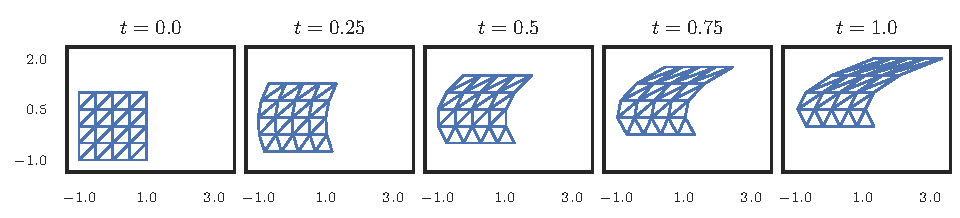
\includegraphics{../images/solution-transfer/mesh_distortion.pdf}
  \centering
  \captionsetup{width=.75\linewidth}
  \caption{Distortion of a regular mesh caused by particle motion along
    the velocity field \(\left[ y^2 \; 1 \right]^T\) from \(t = 0\)
    to \(t = 1\) with \(\Delta t = 1/4\).}
  \label{fig:mesh-distortion}
\end{figure}

A flow-based change to a mesh can cause problems if it causes the mesh to
leave the domain being analyzed or if it distorts the mesh until the element
quality is too low in some mesh elements. Over enough time, the mesh can
even tangle (i.e. elements begin to overlap).
For an example of such distortion (Figure~\ref{fig:mesh-distortion}),
consider a PDE of the form
\begin{equation}\label{eq:non-rigid-characteristics}
u_t + \left[ \begin{array}{c} y^2 \\ 1 \end{array}\right] \cdot \nabla u +
  F\left(u, \nabla u\right) = 0.
\end{equation}
The characteristics \(y(t) = y_0 + t, x(t) = x_0 +
\left(y(t)^3 - y_0^3\right)/3\)
distort the mesh considerably after just one second.

\begin{figure}
  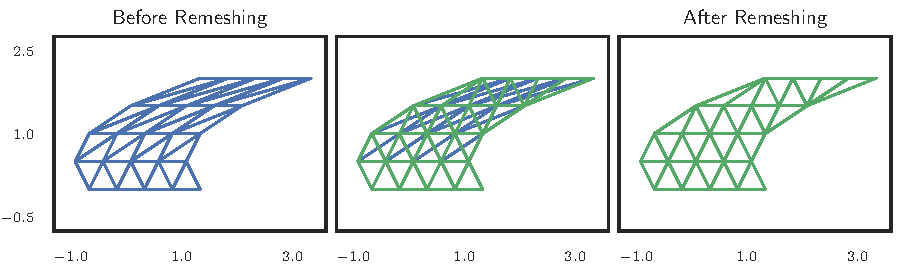
\includegraphics{../images/solution-transfer/distortion_remesh.pdf}
  \centering
  \captionsetup{width=.75\linewidth}
  \caption{Remeshing a domain after distortion caused by particle motion
    along the velocity field \(\left[ y^2 \; 1 \right]^T\) from \(t = 0\)
    to \(t = 1\).}
  \label{fig:distortion-remesh}
\end{figure}

To deal with distortion, one can allow the mesh to adapt in between time
steps. For example, Figure~\ref{fig:distortion-remesh} shows an example
remeshing of the domain.
In addition to improving mesh quality, mesh
adaptivity can be used to dynamically focus computational effort to resolve
sensitive features of a numerical solution. From \cite{Iske2004}
\begin{quote}
{\small In order to balance the method's approximation quality and its
computational costs effectively, adaptivity is an essential requirement,
especially when modelling multiscale phenomena.}
\end{quote}
For more on mesh adaptivity, see \cite{Babuska1978, Peraire1987, Pain2001}.

In either case, the change in the
mesh between time steps requires transferring a known solution on the
discarded mesh to the mesh produced by the remeshing process. Without
the ability to change the mesh, Lagrangian methods (or, more generally,
ALE \cite{Hirt1974}) would not be useful, since after a limited time the
mesh will distort.

\subsection{High-order Meshes}

\begin{figure}
  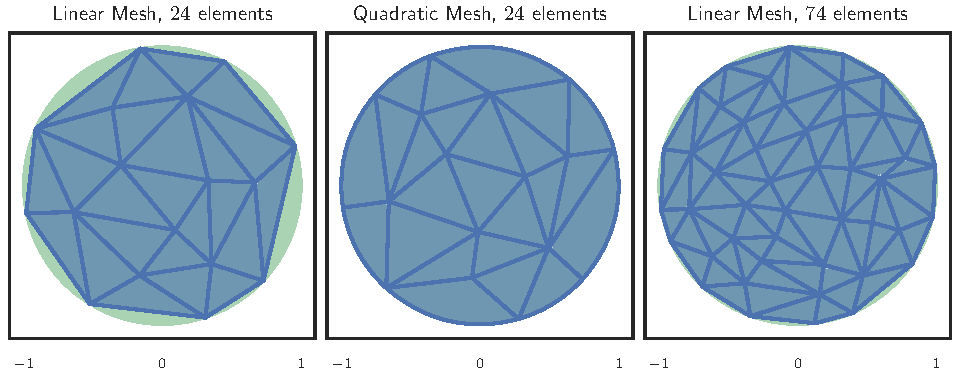
\includegraphics{../images/solution-transfer/main_figure27.pdf}
  \centering
  \captionsetup{width=.75\linewidth}
  \caption{Comparing straight sided meshes to a curved mesh when approximating
    the unit disc in \(\reals^2\).}
  \label{fig:curved-vs-straight-mesh}
\end{figure}

To allow for greater geometric flexibility and for high order of convergence,
curved mesh elements can be used in the finite element method. Though the
complexity of a method can steeply rise when allowing curved elements, the
trade for high-order convergence can be worth it. (See \cite{Wang2013} for
more on high-order CFD methods.) Curved meshes can typically
represent a given geometry with far fewer elements than a straight sided mesh
(for example, Figure~\ref{fig:curved-vs-straight-mesh}).
The increase in accuracy also allows for the use of fewer elements, which
in turn can also facilitate a reduction in the overall computation time.

\begin{figure}
  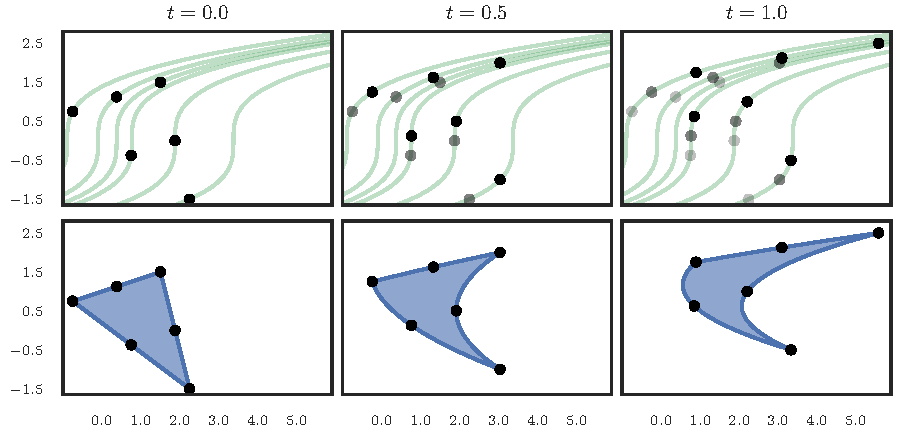
\includegraphics{../images/solution-transfer/element_distortion.pdf}
  \centering
  \captionsetup{width=.75\linewidth}
  \caption{Movement of nodes in a quadratic element under distortion caused
    by particle motion along the velocity field \(\left[ y^2 \; 1 \right]^T\)
    from \(t = 0\) to \(t = 1\) with \(\Delta t = 1/2\). The green curves
    represent the characteristics that each node travels along.}
  \label{fig:element-distortion}
\end{figure}

Even if the domain has no inherent curvature, high-order (degree \(p\)) shape
functions allow for order \(p + 1\) convergence, which is desirable in
it's own right. However, even in such cases, a Lagrangian method must either
curve the mesh or information about the flow of the geometry will be lost.
Figure~\ref{fig:element-distortion} shows what happens to a given
quadratic element as the nodes move along the
characteristics from~\eqref{eq:non-rigid-characteristics}.
This element uses the triangle vertices and edge
midpoints to determine the shape functions. However, as the nodes move
with the flow, the midpoints are no longer on the lines connecting
the vertex nodes. To allow the mesh to more accurately represent the
solution, the edges can instead curve so that the midpoint nodes remain
halfway between (i.e. half of the parameter space) the vertex nodes along
an edge.

\subsection{Multiphysics and Comparing Methods}

In multiphysics simulations, a problem is partitioned into physical components.
This partitioning can apply to both the physical domain (e.g. separating a
solid and fluid at an interface) and the simulation solution itself (e.g.
solving for pressure on one mesh and velocity on another). Each (multi)physics
component is solved for on its own mesh. When the components interact, the
simulation solution must be transferred between those meshes.

In a similar category of application, solution transfer enables the comparison
of solutions defined on different meshes. For example, if a reference
solution is known on a very fine special-purpose mesh, the error can be
computed for a coarse mesh by transferring the solution from the fine
mesh and taking the difference. Or, if the same method is used on
different meshes of the same domain, the resulting computed solutions can
be compared via solution transfer. Or, if two different methods use two
different meshes of the same domain.

\subsection{Local versus Global Transfer}

Conservative solution transfer has been around since the advent of ALE,
and as a result much of the existing literature focuses on mesh-mesh
pairs that will occur during an ALE-based simulation. When flow-based
mesh distortion occurs, elements are typically ``flipped'' (e.g. a
diagonal is switched in a pair of elements) or elements are subdivided
or combined. These operations are inherently local, hence the solution
transfer can be done locally across known neighbors. Typically, this
locality is crucial to solution transfer methods. In \cite{Margolin2003},
the transfer is based on partitioning elements of the updated mesh into
components of elements from the old mesh and ``swept regions'' from
neighbouring elements. In \cite{Kucharik2008}, the (locally) changing
connectivity of the mesh is addressed. In \cite{Garimella2007}, the
local transfer is done on polyhedral meshes.

Global solution transfer instead seeks to conserve the solution across
the whole mesh. It makes no assumptions about the relationship between
the donor and target meshes. The loss in local information makes
the mesh intersection problem more computationally expensive, but the
added flexibility reduces timestep restrictions since it allows remeshing
to be done less often. In \cite{Dukowicz1984, Dukowicz1987}, a global
transfer is enabled by transforming volume integrals to surface integrals
via the divergence theorem to reduce the complexity of the problem.

\subsection{Limitations}

\begin{figure}
  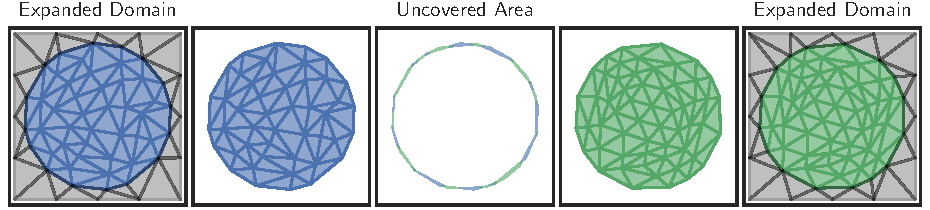
\includegraphics{../images/solution-transfer/main_figure29.pdf}
  \centering
  \captionsetup{width=.75\linewidth}
  \caption{Partially overlapping meshes on a near identical domain. Both are
    linear meshes that approximate the unit disc in \(\reals^2\). The outermost
    columns show how the domain of each mesh can be expanded so they agree.}
  \label{fig:partially-overlapping}
\end{figure}

The method described in this work only applies to meshes in \(\reals^2\).
Application to meshes in \(\reals^3\) is a direction for future research,
though the geometric kernels (see Chapter~\ref{chap:bezier-intersection})
become significantly more challenging to describe and implement. In
addition, the method will assume that every element in the
target mesh is contained in the donor mesh. This ensures that the solution
transfer is \emph{interpolation}. In the case where all target elements are
partially covered, \emph{extrapolation} could be used to extend a solution
outside the domain, but for totally uncovered elements there is no clear
correspondence to elements in the donor mesh.

The case of partially overlapping meshes can be addressed in particular
cases (i.e. with more information). For example, consider a problem
defined on \(\Omega = \reals^2\) and solution
that tends towards zero as points tend to infinity. A typical approach
may be to compute the solution on a circle of large enough radius and
consider the numerical solution to be zero outside the circle.
Figure~\ref{fig:partially-overlapping} shows how solution transfer could be
performed in such cases when the meshes partially overlap: construct a
simple region containing both computational domains and then mesh the
newly introduced area. However, the assumption that the numerical solution
is zero in the newly introduced area is very specific and
a similar approach may not apply in other cases of partial overlap.

Some attempts (\cite{Berger1987, Chesshire1994, Cai1999}) have been
made to interpolate fluxes between overlapping meshes. These perform
an interpolation on the region common to both meshes and then numerically
solve the PDE to determine the values on the uncovered elements.

When solving some PDEs with viscoelastic fields, additional nodes must be
tracked at quadrature points. As the mesh travels, these quadrature points
must be moved as well in a way that is consistent with the standard
nodes that define the element. The solution transfer method described here
does not provide a way either to determine quadrature points on a
target mesh or to map the field onto known quadrature points.

\section{Galerkin Projection}

\begin{figure}
  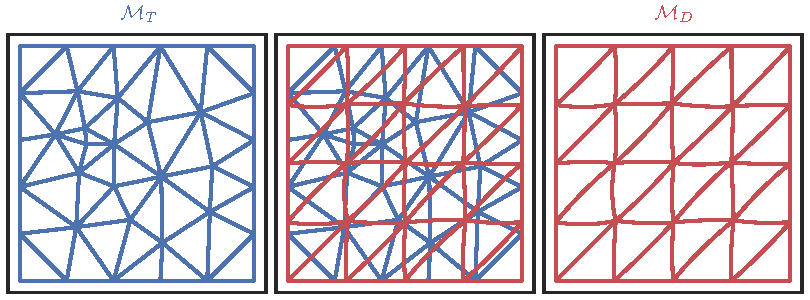
\includegraphics{../images/solution-transfer/main_figure00.pdf}
  \centering
  \captionsetup{width=.75\linewidth}
  \caption{Mesh pair: donor mesh \(\mathcal{M}_D\) and
    target mesh \(\mathcal{M}_T\).}
  \label{fig:donor-target-pair}
\end{figure}

Consider a donor mesh \(\mathcal{M}_D\) with shape function basis
\(\phi_D^{(j)}\) and a known field \(\bm{q}_D = \sum_j d_j \phi_D^{(j)}\)
\footnote{This is somewhat a simplification. In the CG case,
some coefficients will be paired with multiple shape functions, such
as the coefficient at a vertex node.}
and a
target mesh \(\mathcal{M}_T\) with shape function basis \(\phi_T^{(j)}\)
(Figure~\ref{fig:donor-target-pair}).
Each shape function \(\phi\) corresponds to a
given isoparametric curved element (see Section~\ref{sec:curved-elements})
\(\mathcal{T}\) in one of these meshes and has
\(\operatorname{supp}(\phi) = \mathcal{T}\).
Additionally, the shape functions are polynomial degree \(p\) (see
Section~\ref{subsec:shape-functions} for a discussion of shape functions),
but the degree of the donor mesh need not be the same as that of the
target mesh. We assume that both meshes cover the same domain \(\Omega \subset
\reals^2\), however we really only require the donor mesh to cover the
target mesh.

We seek the \(L_2\)-optimal interpolant \(\bm{q}_T = \sum_j t_j \phi_T^{(j)}\):
\begin{equation}
\left \lVert \bm{q}_T - \bm{q}_D \right \rVert_2 =
\min_{\bm{q} \in \mathcal{V}_T}
\left \lVert \bm{q} - \bm{q}_D \right \rVert_2
\end{equation}
where \(\mathcal{V}_T = \operatorname{Span}_j\left\{\phi_T^{(j)}\right\}\)
is the function space defined on the target mesh. Since this is optimal in
the \(L_2\) sense, by differentiating with respect to each \(t_j\) in
\(\bm{q}_T\) we find the weak form:
\begin{equation}
\int_{\Omega} \bm{q}_D \phi_T^{(j)} \, dV =
  \int_{\Omega} \bm{q}_T \phi_T^{(j)} \, dV, \qquad \text{for all } j.
\end{equation}
If the constant function \(1\) is contained in \(\mathcal{V}_T\),
conservation follows from the weak form and linearity of the integral
\begin{equation}
\int_{\Omega} \bm{q}_D \, dV =
  \int_{\Omega} \bm{q}_T \, dV.
\end{equation}
Expanding \(\bm{q}_D\) and \(\bm{q}_T\) with respect to their coefficients
\(\bm{d}\) and \(\bm{t}\), the weak form gives rise to a linear system
\begin{equation}\label{eq:weak-form-system}
M_T \bm{t} = M_{TD} \bm{d}.
\end{equation}
Here \(M_T\) is the mass matrix for
\(\mathcal{M}_T\) given by
\begin{equation}
\left(M_T\right)_{ij} = \int_{\Omega} \phi_T^{(i)} \phi_T^{(j)} \, dV.
\end{equation}
In the discontinuous Galerkin case, \(M_T\) is block diagonal with blocks
that correspond to each element, so \eqref{eq:weak-form-system} can be
solved locally on each element \(\mathcal{T}\) in the target mesh. By
construction, \(M_T\) is symmetric and sparse since \(\left(M_T\right)_{ij}\)
will be \(0\) unless \(\phi_T^{(i)}\) and \(\phi_T^{(j)}\) are supported
on the same element \(\mathcal{T}\). In the continuous case, \(M_T\) is
globally coupled since coefficients corresponding to boundary nodes interact
with multiple elements. The matrix \(M_{TD}\) is a ``mixed'' mass matrix
between the target and donor meshes:
\begin{equation}
\left(M_{TD}\right)_{ij} = \int_{\Omega} \phi_T^{(i)} \phi_D^{(j)} \, dV.
\end{equation}
Boundary conditions can be imposed on the system by fixing some coefficients,
but that is equivalent to removing some of the basis functions which may
in term make the projection non-conservative. This is because the removed
basis functions may have been used in \(1 = \sum_j u_j \phi_{T}^{(j)}\).

Computing \(M_T\) is fairly straightforward since the (bidirectional) mapping
from elements \(\mathcal{T}\) to basis functions \(\phi_T^{(j)}\) supported
on those elements is known. When using shape functions in the
global coordinates basis (see Section~\ref{subsec:shape-functions}), the
integrand \(F = \phi_T^{(i)} \phi_T^{(j)}\) will be a polynomial of degree
\(2p\) on \(\reals^2\). The domain of integration \(\mathcal{T}
= b\left(\utri\right)\) is the image of a (degree \(p\)) map \(b(s, t)\)
from the unit triangle. Using substitution
\begin{equation}\label{eq:mass-mat-subst}
\int_{b\left(\utri\right)} F(x, y) \, dx \, dy =
  \int_{\utri} \det(Db) F\left(x(s, t), y(s, t)\right) \, ds \, dt
\end{equation}
(we know the map preserves orientation, i.e. \(\det(Db)\) is positive).
Once transformed this way, a quadrature rule on the unit
triangle (\cite{Dunavant1985}) can be used.

On the other hand, computing \(M_{TD}\) is significantly more
challenging. This requires solving both a geometric problem ---
finding the region to integrate over --- and an analytic
problem --- computing the integrals. The integration can be done with
a quadrature rule, though finding this region is significantly
more difficult.

\section{Common Refinement}

\begin{figure}
  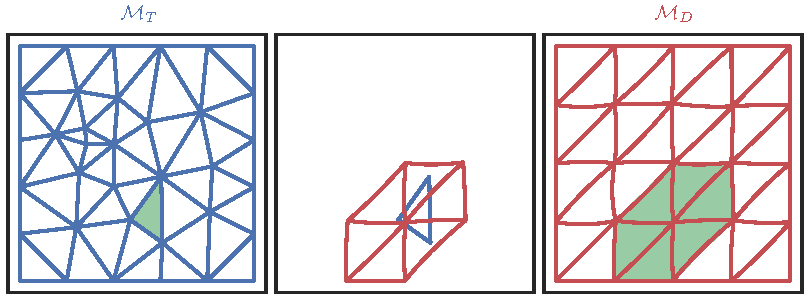
\includegraphics{../images/solution-transfer/main_figure02.pdf}
  \centering
  \captionsetup{width=.75\linewidth}
  \caption{All donor elements that cover a target element}
  \label{fig:target-elt-all-matching}
\end{figure}

Rather than computing \(M_{TD}\), the right-hand side
of~\eqref{eq:weak-form-system} can be computed directly via
\begin{equation}\label{eq:lumped-mixed-mass-matrix}
\left(M_{TD} \bm{d}\right)_j = \int_{\Omega} \phi_T^{(j)} \bm{q}_D \, dV.
\end{equation}
Any given \(\phi\) is supported on an element \(\mathcal{T}\) in the
target mesh. Since \(\bm{q}_D\) is piecewise defined over each element
\(\mathcal{T}'\) in the donor mesh, the
integral~\eqref{eq:lumped-mixed-mass-matrix} may be problematic.
In the continuous Galerkin case, \(\bm{q}_D\) need not be differentiable
across \(\mathcal{T}\) and in the discontinuous Galerkin case,
\(\bm{q}_D\) need not even be continuous. This necessitates a
partitioning of the domain:
\begin{equation}
\int_{\Omega} \phi \, \bm{q}_D \, dV =
  \int_{\mathcal{T}} \phi \, \bm{q}_D \, dV =
  \sum_{\mathcal{T}' \in \mathcal{M}_D} \int_{\mathcal{T} \cap \mathcal{T}'}
    \phi \left.\bm{q}_D\right|_{\mathcal{T}'} \, dV.
\end{equation}
In other words, the integral over \(\mathcal{T}\) splits into integrals
over intersections \(\mathcal{T} \cap \mathcal{T}'\) for all
\(\mathcal{T}'\) in the donor mesh that intersect \(\mathcal{T}\)
(Figure~\ref{fig:target-elt-all-matching}). Since both \(\phi\) and
\(\left.\bm{q}_D\right|_{\mathcal{T}'}\) are polynomials on
\(\mathcal{T} \cap \mathcal{T}'\), the integrals will be exact when
using a quadrature scheme of an appropriate degree of accuracy.
Without partitioning \(\mathcal{T}\), the integrand is not a polynomial
(in fact, possibly not smooth), so the quadrature cannot be exact.

In order to compute \(M_{TD} \bm{d}\), we'll need to compute the
\emph{common refinement}, i.e. an intermediate mesh that contains
both the donor and target meshes. This will consist of all non-empty
\(\mathcal{T} \cap \mathcal{T}'\) as \(\mathcal{T}\) varies over
elements of the target mesh and \(\mathcal{T}'\) over elements of the
donor mesh. This requires solving three specific subproblems:
\begin{itemize}
%% H/T: https://tex.stackexchange.com/a/6086/32270
\itemsep 0em
\item Forming the region(s) of intersection between two elements that
  are B\'{e}zier triangles.
\item Finding all pairs of elements, one each from the target and donor mesh,
  that intersect.
\item Numerically integrating over a region of intersection between two
  elements.
\end{itemize}
The first subproblem has been addressed in Section~\ref{sec:intersect-bez-tri}
and the curved polygon region(s) of intersection have been described
in Section~\ref{subsec:curved-polygons}. The second will be considered
in Section~\ref{subsec:advancing-front} and the third in
Section~\ref{subsec:integration-on-curved} below.

\subsection{Advancing Front}\label{subsec:advancing-front}

\begin{figure}
  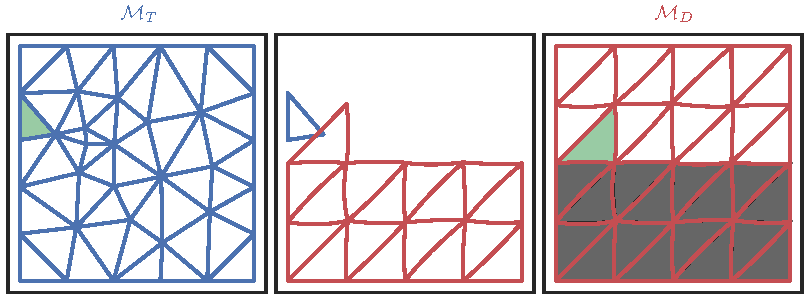
\includegraphics{../images/solution-transfer/main_figure13.pdf}
  \centering
  \captionsetup{width=.75\linewidth}
  \caption{Brute force search for a donor element \(\mathcal{T}'\) that matches
    a fixed target element \(\mathcal{T}\).}
  \label{fig:target-elt-brute-force}
\end{figure}

We seek to identify all pairs \(\mathcal{T}\) and \(\mathcal{T}'\) of
intersecting target and donor elements. The na\"{i}ve approach just
considers every pair
of elements and takes \(\bigO{\left|\mathcal{M}_D\right|
\left|\mathcal{M}_T\right|}\) to complete.\footnote{For a mesh \(\mathcal{M}\),
the expression \(\left|\mathcal{M}\right|\) represents the number of elements
in the mesh.} Taking after \cite{Farrell2011}, we can do much better than this
quadratic time search. In fact, we can compute all integrals in
\(\bigO{\left|\mathcal{M}_D\right| + \left|\mathcal{M}_T\right|}\).
First, we fix an element of the target mesh and perform a brute-force search
to find an intersecting element in the donor mesh
(Figure~\ref{fig:target-elt-brute-force}). This has worst-case time
\(\bigO{\left|\mathcal{M}_D\right|}\).

\begin{figure}
  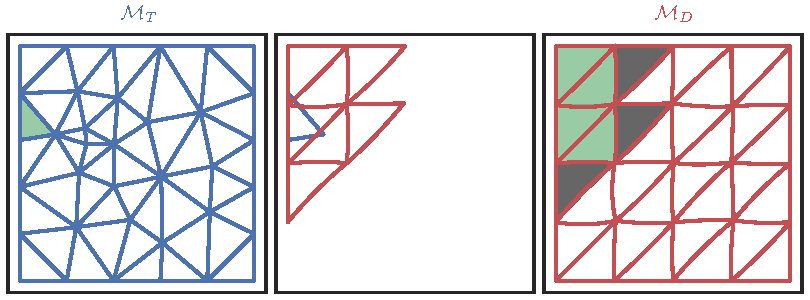
\includegraphics{../images/solution-transfer/main_figure14.pdf}
  \centering
  \captionsetup{width=.75\linewidth}
  \caption{All donor elements \(\mathcal{T}'\) that cover a target element
    \(\mathcal{T}\), with an extra layer of neighbors in the donor mesh
    that \emph{do not} intersect \(\mathcal{T}\).}
  \label{fig:target-elt-overlap-extra-layer}
\end{figure}

Once we have such a match, we use the connectivity graph of the
donor mesh to perform a breadth first search
for neighbors that also intersect the target
element \(\mathcal{T}\) (Figure~\ref{fig:target-elt-overlap-extra-layer}).
This search takes \(\bigO{1}\) time. It's also worthwhile to keep the first
layer of donor elements that don't intersect \(\mathcal{T}\) because they are
more likely to intersect the neighbors of \(\mathcal{T}\)\footnote{In the
very unlikely case that the boundary of \(\mathcal{T}\)
\emph{exactly matches} the boundaries of the donor elements that cover it,
\emph{none} of the overlapping donor elements can intersect the neighbors of
\(\mathcal{T}\) so the first layer of non-intersected donor
elements must be considered.}. Using the list of intersected elements, a
neighbor of \(\mathcal{T}\) can find a donor element it intersects with in
\(\bigO{1}\) time (Figure~\ref{fig:target-elt-neighbor}).
As seen, after our \(\bigO{\left|\mathcal{M}_D\right|}\)
initial brute-force search, the localized intersections for each
target element \(\mathcal{T}\) take
\(\bigO{1}\) time. So together, the process takes
\(\bigO{\left|\mathcal{M}_D\right| + \left|\mathcal{M}_T\right|}\).

For special cases, e.g. ALE methods, the initial brute-force search
can be reduced to \(\bigO{1}\). This could be enabled by tracking
the remeshing process so a correspondence already exists. If a full
mapping from donor to target mesh exists, the process of computing
\(M_T\) and \(M_{TD} \bm{d}\) can be fully parallelized across
elements of the target mesh, or even across shape functions
\(\phi_T^{(j)}\).

\begin{figure}
  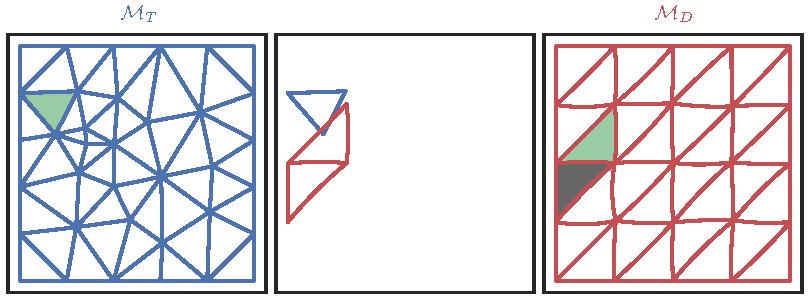
\includegraphics{../images/solution-transfer/main_figure15.pdf}
  \centering
  \captionsetup{width=.75\linewidth}
  \caption{First match between a neighbor of the previously considered
    target element and all the donor elements that match the
    previously considered target element.}
  \label{fig:target-elt-neighbor}
\end{figure}

\subsection{Integration over Curved Polygons}
\label{subsec:integration-on-curved}

In order to numerically evaluate integrals of the form
\begin{equation}
\int_{\mathcal{T}_0 \cap \mathcal{T}_1} F(x, y) \, dV
\end{equation}
we must have a quadrature rule on these curved polygon
(Section~\ref{subsec:curved-polygons}) intersections
\(\mathcal{T}_0 \cap \mathcal{T}_1\).
To do this, we transform the integral into several line integrals
via Green's theorem and then use an exact Gaussian quadrature to
evaluate them. Throughout this section we'll assume the integrand
is of the form \(F = \phi_0 \phi_1\) where each \(\phi_j\) is a shape
function on \(\mathcal{T}_j\). In addition, we'll refer to the two
B\'{e}zier maps that define the elements being intersected:
\(\mathcal{T}_0 = b_0\left(\utri\right)\) and
\(\mathcal{T}_1 = b_1\left(\utri\right)\).

\begin{figure}
  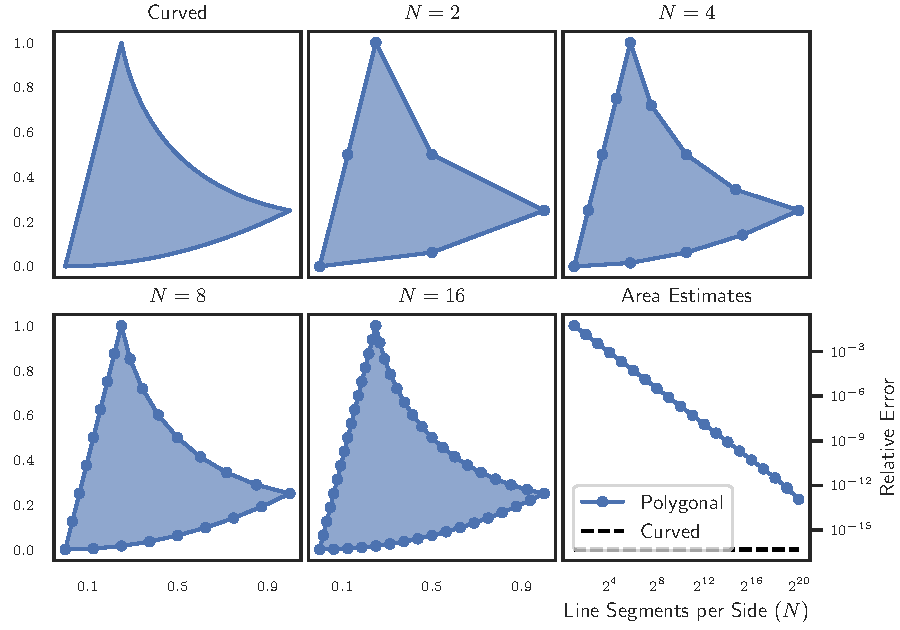
\includegraphics{../images/solution-transfer/polygon_vs_curved.pdf}
  \centering
  \captionsetup{width=.75\linewidth}
  \caption{Comparing the relative error for the computed area of a quadratic
    B\'{e}zier triangle. In one method, the curved boundary is used and the
    result is correct to machine precision. In the other, the curved edges
    are approximated by polygonal paths.}
  \label{fig:polygon-vs-curved}
\end{figure}

\begin{figure}
  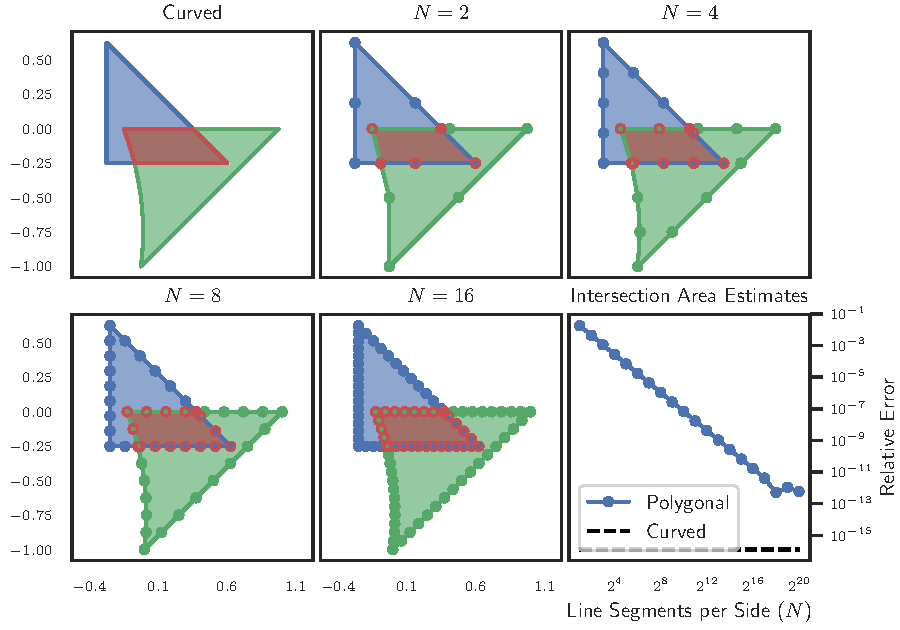
\includegraphics
      {../images/solution-transfer/polygon_vs_curved_intersection.pdf}
  \centering
  \captionsetup{width=.75\linewidth}
  \caption{Comparing the relative error for the computed area of the
    intersection of two quadratic B\'{e}zier triangles. In one method, the
    intersection boundary is fully specified as the union of B\'{e}zier curve
    segments and the area is computed correctly to machine precision. In the
    other, the curved edges are approximated by polygonal paths and the
    intersection of the resulting polygons is computed.}
  \label{fig:polygon-vs-curved-intersection}
\end{figure}

First a discussion of a method not used. A somewhat simple approach would be
be to use polygonal approximation. I.e. approximate the boundary of each
B\'{e}zier triangle with line segments, intersect the resulting polygons,
triangulate the intersection polygon(s) and then numerically integrate
on each triangulated cell. However, this approach is prohibitively inefficient.
For example, consider the curved polygon in
Figure~\ref{fig:polygon-vs-curved}. Computing the area of \(\mathcal{P}\)
can be done via an integral: \(\int_{\mathcal{P}} 1 \, dV\).
By using the actual curved boundary, this integral can be computed with
relative error (the dashed line in the bottom right subplot) on the order
of machine precision \(\bigO{\mach}\). On the other hand, approximating
each side of \(\mathcal{P}\) with \(N\) line segments, the relative error is
\(\bigO{1/N^2}\). (For example, if \(N = 2\) an edge curve \(b(s, 0)\) would be
replaced by segments connecting \(b(0, 0), b(1/2, 0)\) and \(b(1, 0)\), i.e.
\(N + 1\) equally spaced parameters.) This means that in order to perform as
well as an \emph{exact} quadrature used in the curved case, we'd
need \(N = \bigO{1/\sqrt{\mach}}\). Compute the area of \(\mathcal{P}\)
in this way assumes that \(\mathcal{P}\) is already known.
If instead only the B\'{e}zier triangles in the intersection are known, as
in Figure~\ref{fig:polygon-vs-curved-intersection}, the polygonal approach
suffers from the same inefficiency.

Since polygonal approximation is prohibitively expensive,
we work directly with curved edges and compute integrals on a regular
domain via substitution.
If two B\'{e}zier triangles intersect with positive measure, then
the region of intersection is one or more disjoint curved polygons:
\(\mathcal{T}_0 \cap \mathcal{T}_1 = \mathcal{P}\) or
\(\mathcal{T}_0 \cap \mathcal{T}_1 = \mathcal{P} \cup
\mathcal{P}' \cup \cdots\).
The second case can be handled in the same way as the first by handling each
disjoint region independently:
\begin{equation}
\int_{\mathcal{T}_0 \cap \mathcal{T}_1} F(x, y) \, dV =
  \int_{\mathcal{P}} F(x, y) \, dV +
  \int_{\mathcal{P}'} F(x, y) \, dV + \cdots.
\end{equation}
Each curved polygon \(\mathcal{P}\) is defined by its boundary, a
piecewise smooth parametric curve:
\begin{equation}
\partial \mathcal{P} = C_1 \cup \cdots \cup C_n.
\end{equation}
This can be thought of as a polygon with \(n\)-sides that happens to
have curved edges.

Quadrature rules for straight sided polygons have been
studied (\cite{Mousavi2009}) though they are not in wide use. Even
if a polygonal quadrature rule was to be employed, a map would need to be
established from a reference polygon onto the curved edges. This map
could then be used with a change of coordinates to move the integral
from the curved polygon to the reference polygon. The problem of extending
a mapping from a boundary to an entire domain has been studied as
transfinite interpolation
(\cite{chenin:tel-00284680, Gordon1982, Perronnet1998}),
barycentric coordinates (\cite{Wachspress1975}) or mean value coordinates
(\cite{Floater2003}). However, these maps aren't typically suitable for
numerical integration because they are either not bijective or increase the
degree of the edges.

\begin{figure}
  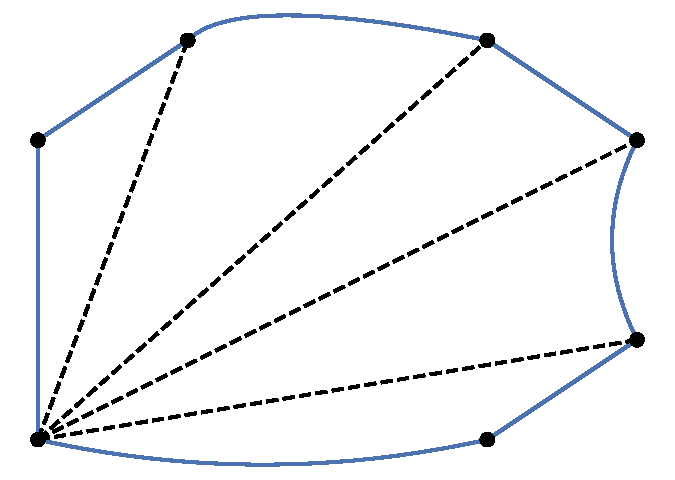
\includegraphics{../images/solution-transfer/main_figure11.pdf}
  \centering
  \captionsetup{width=.75\linewidth}
  \caption{Curved polygon tessellation, done by introducing diagonals
    from a single vertex node.}
  \label{fig:tessellated-curved-polygon}
\end{figure}

Since simple and well established quadrature rules do exist for triangles,
a valid approach would be
to tessellate a curved polygon into valid B\'{e}zier triangles
(Figure~\ref{fig:tessellated-curved-polygon}) and then use substitution as
in~\eqref{eq:mass-mat-subst}. However, tessellation is challenging for both
theoretical and computational reasons.
Theoretical: it's not even clear if an arbitrary curved polygon \emph{can}
be tessellated into B\'{e}zier triangles. Computational: the placement
of diagonals and potential introduction of interior nodes is very
complex in cases where the curved polygon is nonconvex. What's more,
the curved polygon is given only by the boundary, so higher degree triangles
(i.e. cubic and above) introduced during tessellation would need to place
interior control points without causing the triangle to invert. To get a
sense for these challenges, note how the ``simple'' introduction of
diagonals in Figure~\ref{fig:bad-tessellation-required} leads to one
inverted element (the gray element) and another element with area outside
of the curved polygon (the yellow element). Inverted B\'{e}zier triangles
are problematic because the accompanying mapping leaves the boundary
established by the edge curves. For example,
if the tessellation of \(\mathcal{P}\) contains an inverted
B\'{e}zier triangle \(\mathcal{T}_2 = b\left(\utri\right)\) then we'll
need to numerically integrate
\begin{equation}
\int_{\mathcal{T}_2} \phi_0 \phi_1 \, dx \, dy =
  \int_{\utri} \left|\det(Db)\right| \left(\phi_0 \circ b\right)
  \left(\phi_1 \circ b\right) \, ds \, dt.
\end{equation}
If the shape functions are from the pre-image basis (see
Section~\ref{subsec:shape-functions}), then \(\phi_0\)
will not be defined at \(b(s, t) \not\in \mathcal{T}_0\) (similarly for
\(\phi_1\)). Additionally, the absolute value in \(\left|\det(Db)\right|\)
makes the integrand non-smooth since for inverted elements
\(\det(Db)\) takes both signs. If the shape functions are from the
global coordinates basis, then tessellation can be used via an
application of Lemma~\ref{lemma:bad-triangle}, however this involves
more computation than just applying Green's theorem along
\(\partial \mathcal{P}\). By applying the lemma, inverted elements may
be used in a tessellation, for example by introducing artificial
diagonals from a vertex as in Figure~\ref{fig:tessellated-curved-polygon}.
In the global coordinates basis, \(F = \phi_0 \phi_1\) \emph{can}
be evaluated for points in an inverted element that leave
\(\mathcal{T}_0\) or \(\mathcal{T}_1\).

\begin{figure}
  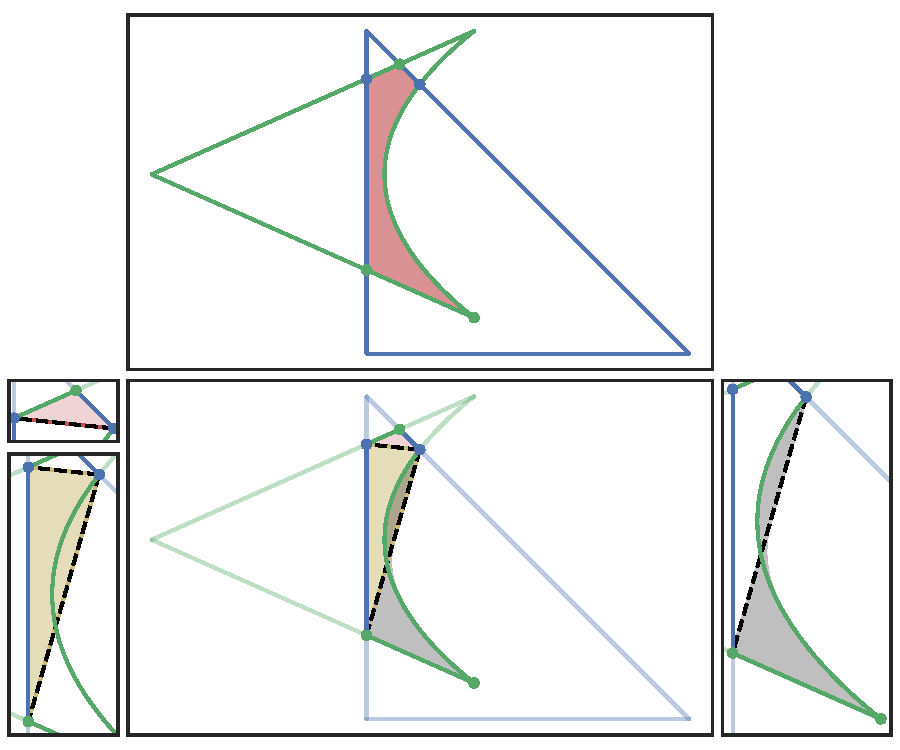
\includegraphics{../images/solution-transfer/main_figure16.pdf}
  \centering
  \captionsetup{width=.75\linewidth}
  \caption{Curved polygon intersection that can't be tessellated
    (with valid B\'{e}zier triangles) by introducing diagonals.}
  \label{fig:bad-tessellation-required}
\end{figure}

Instead, we focus on a Green's theorem based approach.
Define horizontal and vertical antiderivatives
\(H, V\) of the integrand \(F\) such that \(H_x = V_y = F\).
We make these \emph{unique} by imposing the
extra condition that \(H(0, y) \equiv V(x, 0) \equiv 0\).
This distinction is arbitrary, but in order to \emph{evaluate}
\(H\) and \(V\), the univariate functions \(H(0, y)\) and \(V(x, 0)\)
must be specified.
Green's theorem tells us that
\begin{equation}
\int_{\mathcal{P}} 2 F \, dV =
\int_{\mathcal{P}} H_x + V_y \, dV =
\oint_{\partial \mathcal{P}} H \, dy - V \, dx =
\sum_j \int_{C_j} H \, dy - V \, dx.
\end{equation}
For a given curve \(C\) with components \(x(r), y(r)\)
defined on the unit interval, this amounts to having
to integrate
\begin{equation}
G(r) = H(x(r), y(r)) y'(r) - V(x(r), y(r)) x'(r).
\end{equation}
To do this, we'll use Gaussian
quadrature with degree of accuracy sufficient to cover the degree
of \(G(r)\).

If the shape functions are in the global coordinates basis
(Section~\ref{subsec:shape-functions}), then \(G\) will also be a polynomial.
This is because for these shape functions \(F = \phi_0 \phi_1\) will be
polynomial on \(\reals^2\) and so will \(H\) and \(V\) and since each curve
\(C\) is a B\'{e}zier curve segment, the components are also polynomials.
If the shape functions are in the pre-image basis, then \(F\) won't in general
be polynomial, hence the quadrature rules can only be approximate.

To evaluate \(G\), we must also evaluate \(H\) and \(V\) numerically.
For example, since \(H(0, y) \equiv 0\),
the fundamental theorem of calculus tells us that
\(H\left(\alpha, \beta\right) = \int_0^{\alpha} F\left(x, \beta\right) \, dx\).
To compute this integral via Gaussian quadrature
\begin{equation}
H\left(\alpha, \beta\right) \approx \frac{\alpha}{2} \sum_j w_j
  F\left(\frac{\alpha}{2} (x_j + 1), \beta\right)
\end{equation}
we must be able to evaluate \(F\) for
points on the line \(y = \beta\) for \(x\) between \(0\) and \(\alpha\). If
the shape functions are from the pre-image basis, it may not even be possible
to evaluate \(F\) for such points. Since \(\left[\begin{array}{c c} \alpha &
\beta \end{array}\right]^T\) is on the boundary of \(\mathcal{P}\), without
loss of generality
assume it is on the boundary of \(\mathcal{T}_0\). Thus, for some elements
(e.g. if the point is on the bottom of the element), points
\(\left[\begin{array}{c c} \nu & \beta \end{array}\right]^T\) may not be
in \(\mathcal{T}_0\). Since \(\operatorname{supp}(\phi_0) = \mathcal{T}_0\),
we could take \(\phi_0(\nu, \beta) = 0\), but this would make the integrand
non-smooth and so the accuracy of the \emph{exact} quadrature would be
lost. But extending \(\phi_0 = \widehat{\phi}_0 \circ b_0^{-1}\) outside
of \(\mathcal{T}_0\) may be impossible: even though \(b_0\) is bijective on
\(\utri\) it may be many-to-one elsewhere hence \(b_0^{-1}\) can't be
reliably extended outside of \(\mathcal{T}_0\).

Even if the shape functions are from the global coordinates basis,
setting \(H(0, y) \equiv 0\) may introduce quadrature points that
are very far from \(\mathcal{P}\). This can be somewhat addressed by using
\(H(m, y) \equiv 0\) for a suitably chosen \(m\) (e.g. the minimum
\(x\)-value in \(\mathcal{P}\)). Then we have
\(H\left(\alpha, \beta\right) = \int_m^{\alpha} F\left(x, \beta\right) \, dx\).

\section{Numerical Experiments}

\begin{figure}
  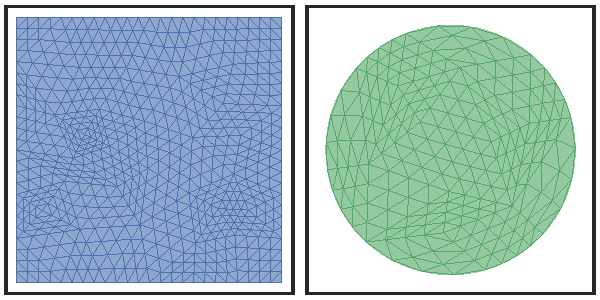
\includegraphics{../images/solution-transfer/main_figure30.pdf}
  \centering
  \captionsetup{width=.75\linewidth}
  \caption{Some example meshes used during the numerical
    experiments; the donor meshs is on the left / blue and the target
    mesh is on the right / green. These meshes are the cubic approximations
    of each domain and have been refined twice.}
  \label{fig:meshes-used-refined}
\end{figure}

A numerical experiment was performed to investigate the observed order
of convergence. Three pairs of random meshes were generated, the donor
on a square of width \(17 / 8\) centered at the origin
and the target on the unit disc. These domains were chosen intentionally so
that the target mesh was completely covered by the donor mesh and the
boundaries did not accidentally introduce ill-conditioned intersection between
elements. The pairs were linear, quadratic and
cubic approximations of the domains. The convergence test was done by
refining each pair of meshes four times and performing solution transfer
at each level. Figure~\ref{fig:meshes-used-refined} shows the cubic
pair of meshes after two refinements.

\begin{figure}
  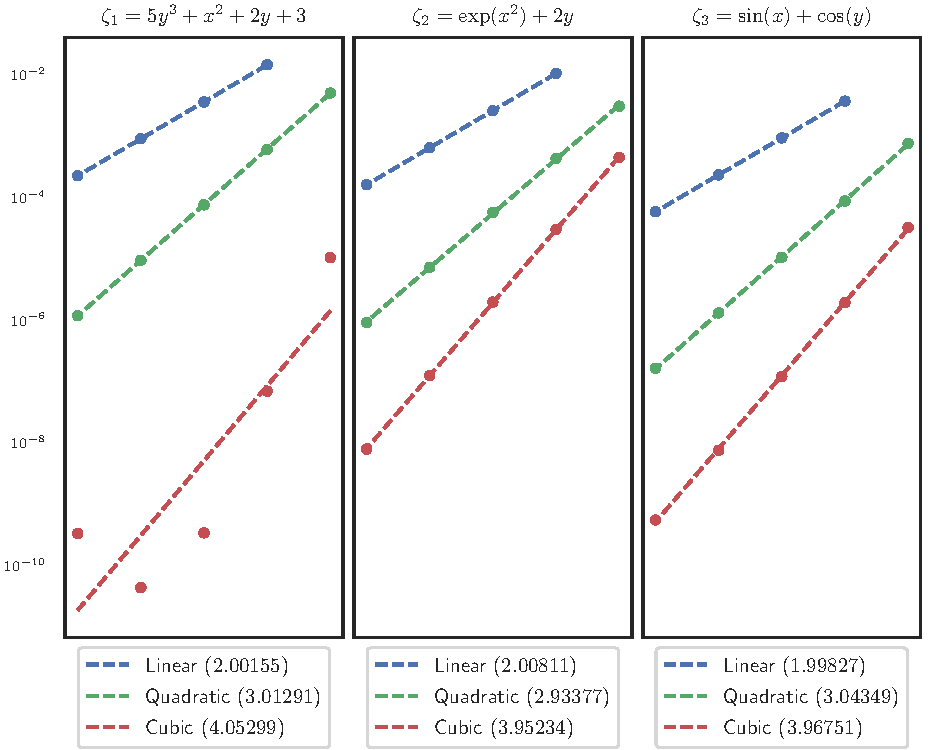
\includegraphics{../images/solution-transfer/main_figure25.pdf}
  \centering
  \captionsetup{width=.75\linewidth}
  \caption{Convergence results for scalar fields on three pairs of related
    meshes: a linear, quadratic and cubic mesh of the same domain.}
  \label{fig:composite-errors}
\end{figure}

Taking after \cite{Farrell2011}, we transfer three
discrete fields in the discontinuous Galerkin (DG) basis.
Each field is derived from one of the smooth scalar functions
\begin{align}
\zeta_1(x, y) &= 5 y^3 + x^2 + 2y + 3 \\
\zeta_2(x, y) &= \exp\left(x^2\right) + 2y \\
\zeta_3(x, y) &= \sin(x) + \cos(y).
\end{align}
For a given mesh size \(h\), we expect that on a degree \(p\) isoparametric
mesh our solution transfer will have \(\bigO{h^{p + 1}}\) errors. To measure
the rate of convergence:
\begin{itemize}
\itemsep 0em
\item Choose a mesh pair \(\mathcal{M}_D\), \(\mathcal{M}_T\) and
a known function \(\zeta(x, y)\).
\item Refine the meshes recursively, starting with
  \(\mathcal{M}_D^{(0)} = \mathcal{M}_D\),
  \(\mathcal{M}_T^{(0)} = \mathcal{M}_T\).
\item Create meshes
\(\mathcal{M}_D^{(j)}\) and \(\mathcal{M}_T^{(j)}\) from
\(\mathcal{M}_D^{(j - 1)}\)
and \(\mathcal{M}_T^{(j - 1)}\) by subdividing each curved
element into four elements.
\item Approximate \(\zeta\) by a discrete field: the nodal
interpolant on the donor mesh \(\mathcal{M}_D^{(j)}\). The
nodal interpolant is constructed by evaluating \(\zeta\) at the
nodes \(\bm{n}_j\) corresponding to each shape function:
\begin{equation}
\bm{f}_j = \sum_i \zeta\left(\bm{n}_i\right) \phi_D^{(i)}.
\end{equation}
\item Transfer \(\bm{f}_j\) to the discrete field \(\bm{g}_j\) on
the target mesh  \(\mathcal{M}_T^{(j)}\).
\item Compute the relative error on \(\mathcal{M}_T^{(j)}\):
\(E_j = \| \bm{g}_j - \zeta \|_2 / \| \zeta \|_2\) (here \(\| \cdot \|_2\)
is the \(L_2\) norm on the target mesh).

We should instead be measuring \(\| \bm{g}_j - \bm{f}_j \|_2 /
\| \bm{f}_j \|_2\), but \(E_j\) is much easier to
compute for \(\zeta(x, y)\) that are straightforward to evaluate.
Due to the triangle inequality \(E_j\) can be a reliable proxy
for the actual projection error, though when
\(\| \bm{f}_j - \zeta \|_2\) becomes too large it will dominate
the error and no convergence will be observed.
\end{itemize}

Convergence results are shown in Figure~\ref{fig:composite-errors}
and confirm the expected orders. Since \(\zeta_1\) is a cubic polynomial,
the solution transfer on the cubic mesh should be \emph{exact}, so there
is a certain minimum threshold that can be reached.
